\chapter{A labeled dataset for analysing deviant orthographic forms in texts written by children}\label{ch:adelaideherci15}
\chapterauthor[1]{Adelaide H.P. Silva}
\chapterauthor[2]{Fabiano Silva}
\chapterauthor[2]{Wanderlan Carvalho}
\chapterauthor[3]{Lourenço Chacon}
\begin{affils}
\chapteraffil[1]{Departamento de Literatura e Linguística, Universidade Federal do Paraná}
\chapteraffil[2]{Departamento de Informática, Universidade Federal do Paraná}
\chapteraffil[3]{Departamento de Fonoaudiologia, Universidade Estadual Paulista}
\end{affils}

%%%%%%%%%%%%%%%%%%%%%%%%%%%%%%%%%%%%%%%%%%%%%%%%%%%%%%%%%%%%%%%%%%%%%%
\section{Introduction}

According to \citet{Chacon2018}, ``writing is a way of enunciating language, that is, a way of putting language to use in a given discursive situation, so that one can learn to write.'' Consequently, individuals have to understand the nature of the language's writing system, that is, its notational system, and also the functioning of the discursive aspects of writing, i.e., its social use. This is the same prediction made by official documents that offer guidelines to the process of teaching Portuguese Language, such as National Common Curriculum Base (BNCC).

We assume, like \citet{Chacon2018}, that orthography, taken as a notational system of a language, must have its operation understood by users so that they can learn to write and thus ``using the language in a given discursive situation''. In other words, learning the spelling of a language is like the first step for users of that language towards learning writing. Hence, the notational system of a language is addressed in the initial years of individuals' formal instruction. Despite being addressed in the early school years, the teaching of spelling is treated mainly, and according to \citet{Morais2000}, as a theme of systematic teaching verification, which results in a lack of planning about the spelling competence expected for students in each school grade. The lack of planning, in turn, is reflected in the absence of guidelines for teaching/learning spelling in the text of the Common National Curriculum Base (BNCC). This scenario causes 33.95\% of students from the 5\textsuperscript{th} grade in Elementary School to show an insufficient level in terms of spelling, according to data from the Ministry of Education, coming from the last National Literacy Assessment, in 2016.

For the above reasons, we started the elaboration of a system that learns the patterns of ``errors'' produced by children in Elementary School, in order to: 1) identify the most recurrent types of ``errors'' in written productions at each level of Elementary School; 2) help teachers to assess the child's performance in the spelling learning process, understanding the hypotheses that children build about the functioning of the language's notation system and identifying aspects to be worked on with the children to improve their performance; 3) help build guidelines for teaching spelling, so that a plan can be drawn up on which aspects to teach in the different grades of Elementary School. The last two points obviously depend on the first one, and are aspects to be developed in secondary or long term. In this work, we will address the identification of patterns of ``errors'' and the grouping of types of ``errors'' \citep{Chacon2018} in the written productions of children from the third and fifth grades of Elementary School. The next section exposes the typology of ``errors'' by \citet{Chacon2018} and the following sections deal with the functioning of the system.

%%%%%%%%%%%%%%%%%%%%%%%%%%%%%%%%%%%%%%%%%%%%%%%%%%%%%%%%%%%%%%%%%%%%%%
\section{A typology of spelling ``errors''}

In designing our system that analyzes non-standard spellings in texts written by children, the first step was to identify the ``errors'' and establish patterns for them. So, it was necessary to analyze an initial set of data in the light of parameters that would help us to recognize the ``errors''. To do so, we turn to \citet{Chacon2018} who offer a typology of ``errors'' in children's written productions.

The authors propose that there is a gradiency in the relationship between the sounds and phonemes of Brazilian Portuguese and the orthographic system. This is a new approach in the literature, which differs from previous ones that predicted categories of ``errors'' (e.g., \citep{Lemle1982, Cagliari1990, Morais2000}). \citet{Chacon2018} propose that there are processes of omissions, transpositions and substitutions. In the first case, we would have, e.g., ``pene'' for ``pente'' (comb); in the second, ``porfessor'' for ``professor'' (teacher) and, in the third, ``sebola'' for ``cebola'' (onion). The authors explain that gradiency is revealed in the fact that, in omissions, there is no orthographic record of a sound, which puts them in a different situation from that of transpositions and substitutions, in which there is an orthographic record of the intended unit to be represented, although in transpositions the grapheme that represents a certain sound is not in the expected position and, in substitutions, the grapheme occupies the expected position, but is itself expected in the representation of a certain sound.

Still with regard to transpositions and substitutions, the authors argue that there is a gradiency within each fact. Thus, transpositions can involve permutations, when there is an exchange of position of two graphemes within a word (eg, ``senera'' for ``serena'', meaning serene), or when there is an exchange of intersyllabic graphemes (eg, ``drento'' for ``dentro'' (inside), in which the change of position of a grapheme affects two syllables) or, even when there is a change of intrasyllabic graphemes and a grapheme moves from one position to another one in the same syllable (eg, ``pregunta'' for ``pergunta'' (question), in which the change position of a grapheme affects a single syllable). With regard to substitutions, \citet{Chacon2018} note that they can be: hybrid substitutions, in cases where a grapheme is replaced by another one that can represent the same phoneme, in another context, such as ``licid'' for ``líquido'', meaning liquid; non-phonological substitutions, in cases where a grapheme is used to represent a sound in a context where it was not anticipated, such as ``rrato'' for ``rato'', i.e, mouse; phonological orthographic substitutions, in cases where the alteration of a grapheme changes what the authors call \emph{phonological value}, as in ``galo'' (rooster) by ``calo'' (callus), in which the sonority of the consonant represented by the initial grapheme of the word is altered. It should be noted that the authors add that phonological orthographic substitutions behave differently from other substitutions and may involve sounds from the same class, as well as sounds from a different class. Thus, e.g., a grapheme substitution representing sound of a distinct class from the target grapheme can be found in ``molacha'' for ``bolacha'' (cookie). The substitutions of graphemes that represent sounds within the same class can be exemplified by the spelling ``gola'' (collar) by ``cola'' (glue).

Table \ref{tab_errors_chacon} illustrates the types of ``errors'' predicted by \citet{Chacon2018}, as well as the subsets of ``errors'' within each type, with examples found in the texts of the dataset which we based our analysis on.

\begin{table}[!ht]
\caption{Typology of ``errors'' from \citep{Chacon2018}.}
\label{tab_errors_chacon}
\centering
\begin{small}
\begin{tabular}{llll}
\hline
\hline
\textit{type} & \textit{subtype} & \textit{example} & \textit{reference} \\
\hline
omission & & redodo & redondo (\textit{round}) \\
\hline
\multirow{3}{*}{transposition}
& permutation   & desromonou & desmoronou (\textit{fell apart})\\
& intersyllabic & despedirça & desperdiça (\textit{he wastes}) \\
& intrasyllabic & quator     & quatro (\textit{four}) \\
\hline
\multirow{3}{*}{substitution}
& hybrid           & cachoro & cachorro (\textit{dog}) \\
& non-phonological & fumasa  & fumaça (\textit{smoke}) \\
& phonological     & futebou & futebol (\textit{soccer}) \\
\hline
\hline
\end{tabular}
\end{small}
\end{table}

%\ade{Colocar aqui a Figura do slide 8}

It is worth considering that the proposal by \citet{Chacon2018} is a work in progress, so it does not include ``errors'' involving vowels or ``errors'' related to prosodic domains, such as the phonological word. For this reason, when analyzing the dataset that we take as a starting point for our system, we established additional categories of ``errors'' that aim to deal with facts such as vowel harmony, e.g. ``repitiu'', for ``repetiu'' (he repeated) or the spelling of a phonological word as a single spelling word, e.g. ``tabom'', for ``está bom'' (ok, then), as well as the reverse, i.e. the spelling of a single phonological word as more than one spelling word, e.g. ``com ver sar'', for ``conversar'' (to talk). Therefore, we established the type ``substitution'', with subsets involving front and posterior vowels, as well as the subset ``random'' that comprises substitutions that involve vowels with no apparent motivation. We also established the type ``others'', that comprise phenomena related to word segmentation, motivated mainly, and apparently, by the notion of phonological word. Besides these types of ``errors'', we also established a type ``insertion'', that deals with the incorporation of an unexpected grapheme into a word, and a type ``combined facts'', that gathers errors from different types within the same word.

Table \ref{tab_errors_add} shows the additional types of ``errors'' we refer to and illustrates them with examples found in the texts of the dataset.

\begin{table}[!ht]
\caption{Additional proposed types of ``errors''.}
\label{tab_errors_add}
\centering
\begin{small}
\begin{tabular}{llll}
\hline
\hline
\textit{type} & \textit{subtype} & \textit{example} & \textit{reference} \\
\hline
\multirow{3}{*}{vowel substitution}
& front     & eli      & ele (\textit{he}) \\
& porterior & pulicial & policial (\textit{policeman}) \\
& random    & uruba    & urubu (\textit{vulture}) \\
\hline
insertion      & & seisi & seis (\textit{six}) \\
\hline
others         & & eamãe & e a mãe (\textit{and the mother})\\
\hline
combined facts & & pasarros & pássaros (\textit{birds})\\
\hline
\hline
\end{tabular}
\end{small}
\end{table}

%\ade{Colocar aqui a Figura do slide 9}

%%%%%%%%%%%%%%%%%%%%%%%%%%%%%%%%%%%%%%%%%%%%%%%%%%%%%%%%%%%%%%%%%%%%%%
\section{Dataset}
The initial set of children's writing data for our system is the written language database assembled by the ``Language Studies Research Group'' (GPEL). The database \citep{Chacon2018} brings together texts produced especially for the constitution of the corpus by children from the first to the fifth year of elementary school in a public school in the city of Marília (SP).

The texts result from a task of retelling a narrative that was read in the classroom by the teacher to the students. This procedure was adopted to all the five school grades that were the target of the database. The initial objective of the UNESP colleagues was to collect four texts from each child in each grade, but this was not possible for all the children, because some of them missed class on the day of one or more collections. In addition, only the texts of children whose parents signed the Informed Consent Term were included in the database. In this initial stage of elaborating the system, we selected the texts of the third and fifth grades, which constitute the end, respectively, the first and second cycles of Elementary School and, therefore, involve the evaluation of children's productions. Due to this methodological decision, our dataset consists of 65 texts from 3\textsuperscript{rd} grade students and 63 texts from 5\textsuperscript{th} grade students, making a total of 128 texts, with 45561 words and 356 words per text, on average.

In addition to selecting a subset of texts for the constitution of our dataset, another methodological decision we made was to adopt orthographic words, and not texts, as the units of analysis. Orthographic words are strings delimited by blank spaces or punctuation marks. Our methodological decision is due to the fact that, as our focus is spelling, taking the word as a unit of analysis allows us to reach the syllable an the segment, two other linguistic units in which ``errors'' manifest themselves (still according to \citet{Chacon2018}).

Once the units of analysis were defined, we made a manual classification of the ``errors'' in each text, following the types  presented in section 2. With the typology of the ``errors" of the dataset, we made a profiling of the data, using Pandas, an open Python library specifically for data analysis.

%%%%%%%%%%%%%%%%%%%%%%%%%%%%%%%%%%%%%%%%%%%%%%%%%%%%%%%%%%%%%%%%%%%%%%
\section{Profilling results and discussion}

The profiling of the ``errors'' in texts of 3\textsuperscript{rd.} grade (Figure \ref{fig_3rd}) reveals that there is a prevalence of the combined facts type in the data. This type of ``error'' refers to occurrences of facts of a different nature in the same word. Thus, e.g., ``enveconhados'', exhibits `r' omission in syllable coda and a phonological substitution that consists in replacing two segments within the same class, that is, `g' by `c'. Omissions are also quite frequent. The ``others'' type, as seen in the histogram, is one of the least frequent.

\begin{figure}[!ht]
\centering
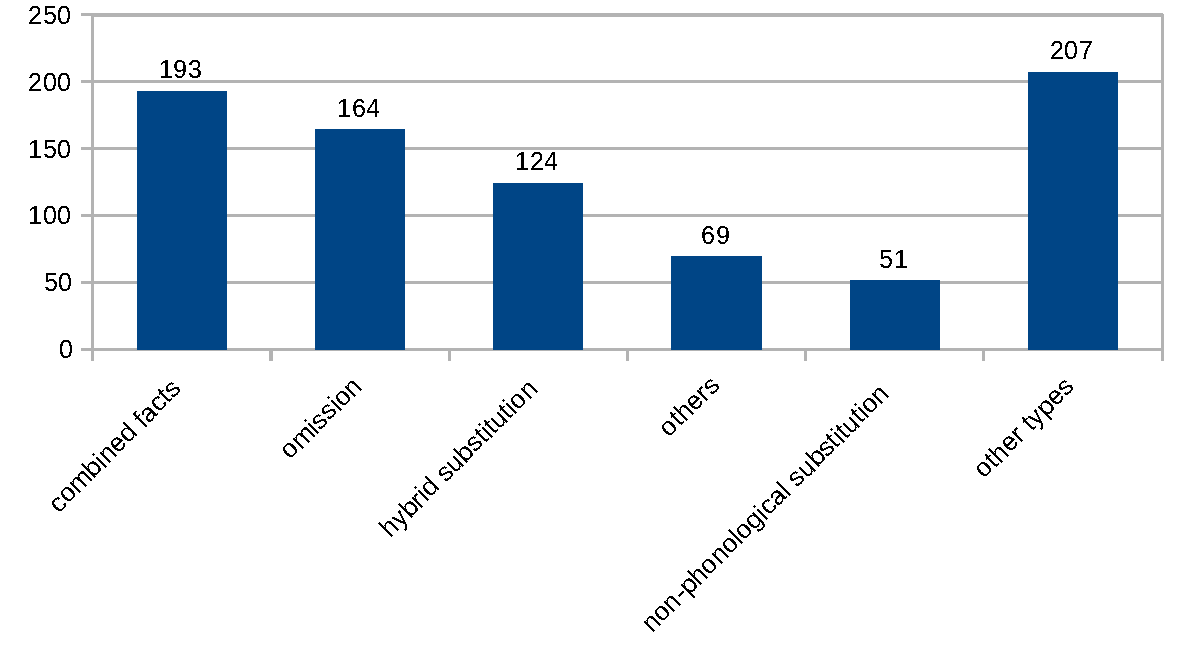
\includegraphics[width=0.95\textwidth]{imgs/adelaideherci15-histograma3.pdf}
\caption{Number of occurrences by type for 3\textsuperscript{rd} grade data.
}
\label{fig_3rd}
\end{figure}

%\ade{Colocar aqui a Figura 1 do texto}

Checking now the distribution of ``errors'' in the texts of 5\textsuperscript{th} grade children, we notice a different distribution of data.

\begin{figure}[!ht]
\centering
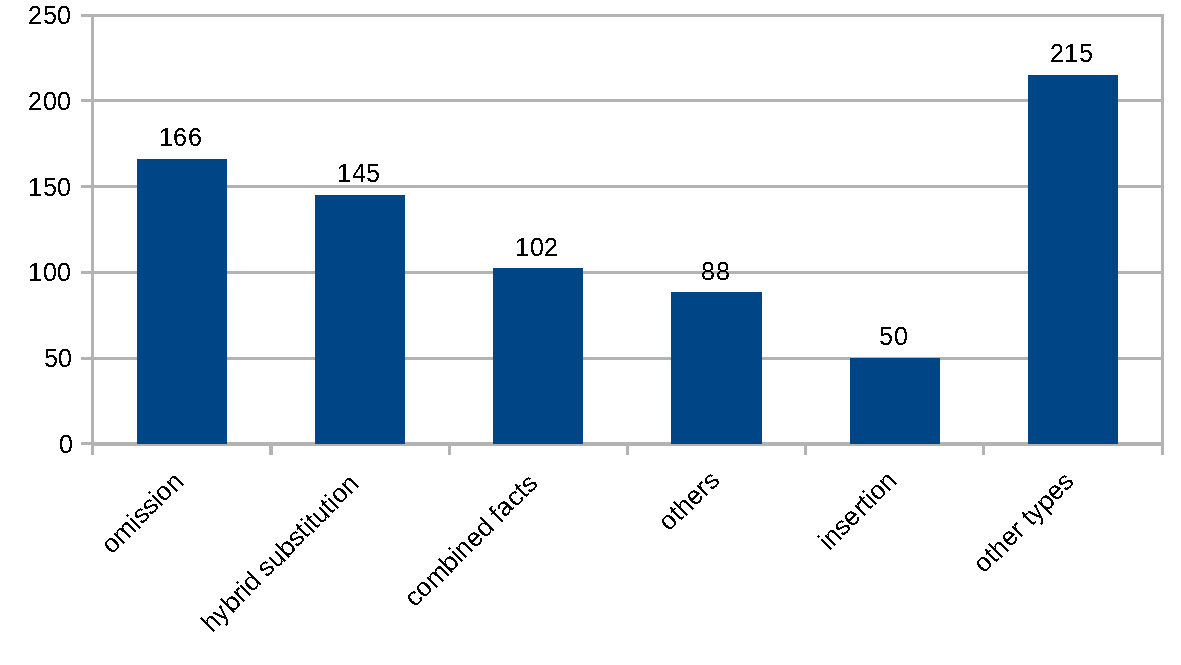
\includegraphics[width=0.95\textwidth]{imgs/adelaideherci15-histograma5.pdf}
\caption{Number of occurrences by type for 5\textsuperscript{th} grade data.
}
\label{fig_5th}
\end{figure}

%\ade{Colocar aqui a Figura 1 do texto}

Figure \ref{fig_5th} shows a decrease in the frequency of occurrence of combined facts in the 5\textsuperscript{th} grade data, compared to the 3\textsuperscript{rd} grade. In the 3\textsuperscript{rd} grade, cases o combined facts account for 24\% of the types of ``errors''; in 5\textsuperscript{th} grade data, by 13\% of them.
On the other hand, the type omission remains very close in both series. An examination of data from the 5\textsuperscript{th} grade reveals that omissions occur mainly in the reduction of diphthongs of the 3\textsuperscript{rd} person, singular, in forms in past perfect tense (e.g., ``assopro'' instead of ``assoprou'', he blew); in the deletion of the `r' of verbal infinitive forms (e.g., ``espirra'', instead of ``espirrar'', to sneeze) or in forms of the verb to be, in which the entire first syllable is deleted, as in ``tava'', instead of ``estava'' (he was). Faced with these cases, the cases of omission in the 3\textsuperscript{rd} grade texts follow another pattern: in them, there is deletion of the grapheme `n', e.g., as a mark of the nasality of the vowel (as in ``ligua'', instead of ``língua'', tongue), or of the `r' in syllable coda (as in ``Macelo'', instead of ``Marcelo''), of the `s' in the same position (as in ``contruir'', instead of ``construir'', to build), or even more than one grapheme, as in ``reportes'', instead of ``repórteres''. These data suggest that, from the 3\textsuperscript{rd} to the 5\textsuperscript{th} grade, omissions are more localized and, to some extent, approximate the written forms to the spoken forms in a colloquial register. During their school time, children seem to learn that a letter is needed to mark the nasality of a vowel, for example. At the same time, they begin to register, in writing, syllabic structures that are more complex than CV.
The others type, in turn, has a different path: it increases from the 3\textsuperscript{rd} to the 5\textsuperscript{th} grade. Interestingly, this kind of ``error'' is related to prosody -- it gathers facts like ``denovo'', instead of ``de novo'' (again) for example. Apparently, children start to build hypotheses about the segmentation of the speech chain more recurrently.

%%%%%%%%%%%%%%%%%%%%%%%%%%%%%%%%%%%%%%%%%%%%%%%%%%%%%%%%%%%%%%%%%%%%%%
\bibliographystyle{plainnat}
\bibliography{adelaideherci15.bib}


